\chapter{The Keyboard and Navigation}
\label{ch:keyboard}

LiNC is built for a CNC panel keyboard: the keys are labelled with what they do at the
machine, not with the letters a PC keyboard happens to send. A normal PC keyboard works
too, and the profile can name the keys either way: \texttt{[ui] keyboard = "panel"} prints
the panel legends, \texttt{[ui] keyboard = "pc"} adds the keys a PC keyboard sends.

Every action in the interface can be reached from the keyboard. Nothing needs a pointer,
nothing needs a touch, and nothing depends on a \keycap{Tab} key.

\section{The navigation column}

\subsection*{The main layer}

The main layer holds what a program is typed from:

\begin{itemize}
  \item the address letters \texttt{O N G X Y Z F D H M S T P Q R} and all ten digits;
  \item \texttt{ENT} to commit, \texttt{BkSp} to delete, \texttt{Space};
  \item the punctuation a program needs: \texttt{. - / ;} and their shifted forms;
  \item the page and cursor keys, and \texttt{Shift} and \texttt{Ctrl};
  \item the five machine keys \pbtn{MAIN}, \pbtn{FILE}, \pbtn{OFFS}, \pbtn{TOOL}, \pbtn{WIN}
        and \pbtn{ESC}.
\end{itemize}

The letters that are rare in G-code -- \texttt{A B C E I J K L U V W} -- are not on the main
layer. They are the blue legends, reached with \keycap{Shift} or a double tap.

\begin{figure}[H]
  \centering
  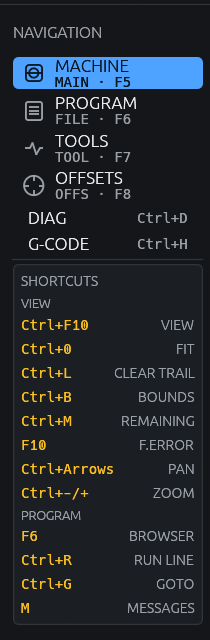
\includegraphics[width=0.24\textwidth]{img/crops/rail.png}
  \caption{The navigation column and the shortcut pane. The shortcut pane lists the keys
           that work on the page in front; it is a reminder, not a set of buttons.}
  \label{fig:rail}
\end{figure}

\begin{longtable}{L{3.4cm}L{2.4cm}L{7.0cm}}
  \toprule
  \textbf{Row} & \textbf{Key} & \textbf{Opens} \\
  \midrule
  \endhead
  \textsf{MACHINE} & \keycap{F5} & The Machine page, or in EDIT/JOG/INC/MPG/HOME the page
        that belongs to the panel mode. \\
  \textsf{PROGRAM} & \keycap{F6} & The Program page. Pressing it again opens the Files
        browser; pressing it in Files brings the program back. \\
  \textsf{TOOLS} & \keycap{F7} & The tool table. \\
  \textsf{OFFSETS} & \keycap{F8} & The work offsets. Pressed again, it moves on to the probe
        tabs, one press per tab, and from the last tab back to Offsets. \\
  \textsf{DIAG} & \chordtwo{Ctrl}{D} & Diagnostics. \\
  \textsf{G-CODE} & \chordtwo{Ctrl}{H} & The G-code help. \\
  \bottomrule
\end{longtable}

The profile may hide rows or change their order, so a machine can ship without the pages it
does not use.

\section{Focus and movement}

The shell has three focus regions: the navigation column, the page, and the page's actions.
The focused element always has a visible ring.

\begin{description}[font=\normalfont\sffamily\bfseries, leftmargin=3.2cm, style=nextline]
  \item[Arrow keys] Move within the current region: rows, table cells, list entries, chips.
  \item[\keycap{Enter}] Activates: open a folder, load a program, commit a cell, issue an MDI
        block, run the highlighted routine.
  \item[\keycap{Esc}] Goes back: closes a dialog, leaves the help article, cancels an edit.
        On any page while a program is active it resets the program.
  \item[\keycap{Home}] / \keycap{End} First and last entry of a list. Inside a text field
        they move to the start and end of the line.
  \item[\keycap{PgUp}] / \keycap{PgDn} A screenful in a list or a read-only program; on
        Diagnostics and the probe tabs, the next tab.
\end{description}

A text field that holds the keyboard keeps the page keys for itself: inside the editor,
\keycap{PgUp} moves the cursor rather than the page.

\section{Keys that work everywhere}

\begin{longtable}{L{4.7cm}L{8.1cm}}
  \toprule
  \textbf{Keys} & \textbf{Action} \\
  \midrule
  \endhead
  \keycap{F5} \dots \keycap{F8} & Navigation, as in the table above. \\
  \chordtwo{Ctrl}{D} & Diagnostics. \\
  \chordtwo{Ctrl}{H} & G-code help. \\
  \keycap{M} & The full-screen messages dialog. \\
  \keycap{Esc} & Back, cancel, or reset the program when one is active. \\
  \chordtwo{Ctrl}{Q} & Quit. Refused while a program runs or an axis moves. \\
  \chordtwo{Ctrl}{O} & Open the Files browser, from any page except Program, where
        \keycap{F6} does it. \\
  \chordtwo{Ctrl}{S} & Save the editor buffer. \\
  \chordtwo{Ctrl}{Z} / \chordtwo{Ctrl}{Y} & Undo / redo in the editor. \\
  \chordtwo{Ctrl}{F} & Search the G-code help (Help page only). \\
  \chordthree{Ctrl}{Shift}{O} & Toggle the limit-switch override. \\
  \bottomrule
\end{longtable}

\begin{cautionbox}
  \chordtwo{Ctrl}{Q} ends the session. It is refused while the machine is busy on
  purpose: a quit prompt in the middle of a cut is a dialog in the way.
\end{cautionbox}

\section{Keys for the toolpath}

Every page that draws a toolpath answers the same view keys, so a view command learned on
one page works on the next.

\begin{longtable}{L{4.7cm}L{8.1cm}}
  \toprule
  \textbf{Keys} & \textbf{Action} \\
  \midrule
  \endhead
  \chordtwo{Ctrl}{F10} & Cycle the view: ISO, X, Y, Z. A lathe toggles ISO and its XZ
        view. \\
  \chordtwo{Ctrl}{0} & Fit the drawing to the page. \\
  \chordtwo{Ctrl}{L} & Clear the live tool trail only. \\
  \chordtwo{Ctrl}{B} & Cycle the bounds: program dimensions, machine envelope, program
        box, off. \\
  \chordtwo{Ctrl}{M} & REMAINING: show only what is still to run. \\
  \keycap{Ctrl}+arrows & Pan the view. \\
  \chordtwo{Ctrl}{+} / \chordtwo{Ctrl}{-} & Zoom in / out. \\
  \bottomrule
\end{longtable}

The pointer does the same: dragging pans, the wheel zooms, a middle-drag orbits in 3D, and a
double click returns to the default isometric view. On the keyboard, \chordtwo{Ctrl}{F10}
and \chordtwo{Ctrl}{0} cover the two commands that matter most.

\section{Keys for programs and the editor}

\begin{longtable}{L{4.7cm}L{8.1cm}}
  \toprule
  \textbf{Keys} & \textbf{Action} \\
  \midrule
  \endhead
  \chordtwo{Ctrl}{R} & RUN FROM LINE: start the loaded program at the selected line. \\
  \chordtwo{Ctrl}{G} & GO TO LINE: ask for a line number and move the view there. \\
  \chordtwo{Ctrl}{U} & UNLOAD: close the program and release the network interlock. \\
  \keycap{F10} & Toggle the Program layout: SPLIT and CODE. \\
  \chordtwo{Ctrl}{\textuparrow} / \chordtwo{Ctrl}{\textdownarrow} & Move the selected line up or down in
        the editor. \\
  \chordtwo{Ctrl}{\textleftarrow} / \chordtwo{Ctrl}{\textrightarrow} & Move by word in the editor and the
        MDI input. \\
  \chordtwo{Ctrl}{A} / \keycap{C} / \keycap{X} / \keycap{V} & Select all, copy, cut,
        paste in the editor. \\
  \chordtwo{Ctrl}{K} & Delete the current line in the editor. \\
  \chordtwo{Ctrl}{D} & Duplicate the current line in the editor. It shadows the
        Diagnostics key while the editor has the keyboard. \\
  \bottomrule
\end{longtable}

\begin{notebox}
  \chordtwo{Ctrl}{R} has three page-local meanings: run from line on Program, run the
  selected block in the MDI pane, and refresh the listing in Files. The shortcut pane always
  shows the one that applies now.
\end{notebox}

\section{Reading the shortcut pane}

The pane under the navigation column lists the page's own keys in groups: \state{VIEW},
\state{PROGRAM}, \state{BROWSE}, \state{FILE}, \state{MEDIA}, \state{LOG VIEW},
\state{PROBE KEYS} and so on. Each line is a key or chord on the left and the action it
performs on the right. The list changes with the page and with the state: while the MDI pane
is up it lists the MDI keys instead of the program keys, and while the editor holds the
keyboard it lists the line-move chords.

When the pane shows nothing, the page has no page-local keys. The global keys above still
work.

\section{Dialogs}

A dialog owns the keyboard while it is open. \keycap{Enter} confirms, \keycap{Esc} cancels,
the arrows move between its buttons or fields, and nothing behind it reacts to a key. The
messages dialog scrolls with \keycap{PgUp}/\keycap{PgDn} and closes with \keycap{Enter} or
\keycap{Esc}.

The unsaved-changes dialog has no third option: save, discard, or cancel the action that
would have thrown the buffer away. Saving is greyed out when a condition blocks it, and the
dialog names the condition.

\clearpage
\section{The CNC keyboard}
\label{sec:cnckeyboard}

The machine keyboard is a 48-key USB keyboard with per-key RGB backlight. Its layout is the
industrial-controller layout: the letters and digits a G-code program is written from sit on
the main layer, and everything else is reached with \keycap{Shift} or by tapping a key twice.
The bottom row carries the navigation keys, so the whole interface is within one hand's reach.

\begin{figure}[H]
  \centering
  \begin{tikzpicture}
    % row 0
    \kbkey{0}{0}{O}{A}   \kbkey{1}{0}{N}{B}   \kbkey{2}{0}{G}{C}
    \kbkey{3}{0}{7}{\%}  \kbkey{4}{0}{8}{@}   \kbkey{5}{0}{9}{\#}
    % row 1
    \kbkey{0}{1}{X}{U}   \kbkey{1}{1}{Y}{V}   \kbkey{2}{1}{Z}{W}
    \kbkey{3}{1}{4}{\$}  \kbkey{4}{1}{5}{:}   \kbkey{5}{1}{6}{=}
    % row 2
    \kbkey{0}{2}{F}{E}   \kbkey{1}{2}{D}{L}   \kbkey{2}{2}{H}{[}
    \kbkey{3}{2}{1}{]}   \kbkey{4}{2}{2}{<}   \kbkey{5}{2}{3}{>}
    % row 3
    \kbkey{0}{3}{M}{I}   \kbkey{1}{3}{S}{J}   \kbkey{2}{3}{T}{K}
    \kbkey{3}{3}{.}{,}   \kbkey{4}{3}{0}{\textbackslash} \kbkey{5}{3}{-}{+}
    % row 4
    \kbkey{0}{4}{P}{(}   \kbkey{1}{4}{Q}{)}   \kbkey{2}{4}{R}{\&}
    \kbkey{3}{4}{/}{*}   \kbkey{4}{4}{;}{\_}  \kbkey{5}{4}{ENT}{m1}
    % row 5
    \kbkey{0}{5}{PgUp}{} \kbkey{1}{5}{Home}{} \kbkey{2}{5}{\textuparrow}{m\,\textuparrow}
    \kbkey{3}{5}{End}{}  \kbkey{4}{5}{Space}{} \kbkey{5}{5}{BkSp}{tetris}
    % row 6
    \kbkey{0}{6}{PgDn}{} \kbkey{1}{6}{\textleftarrow}{m\,\textleftarrow}
    \kbkey{2}{6}{\textdownarrow}{m\,\textdownarrow}
    \kbkey{3}{6}{\textrightarrow}{m\,\textrightarrow}
    \kbkey{4}{6}{SHIFT}{} \kbkey{5}{6}{Ctrl}{}
    % row 7
    \kbkey{0}{7}{MAIN}{F5} \kbkey{1}{7}{FILE}{F6} \kbkey{2}{7}{OFFS}{F8}
    \kbkey{3}{7}{TOOL}{F7} \kbkey{4}{7}{WIN}{F10} \kbkey{5}{7}{ESC}{}
  \end{tikzpicture}
  \caption{Keyboard layout. Centre: the main layer. Small blue legends: the shift and
           double-tap layer (\texttt{m} = mouse key).}
  \label{fig:keyboard}
\end{figure}


\subsection*{Shift and double tap}

\begin{description}[font=\normalfont\sffamily\bfseries, leftmargin=2.6cm, style=nextline]
  \item[\keycap{Shift}] Hold it, then press the key: the blue legend is sent. The dual-layer
        keys glow brighter blue while Shift is held.
  \item[Double tap] Tap the same key twice within 0.3\,s. The first character is erased and
        the blue legend is written instead: \keycap{O}\,\keycap{O} writes \texttt{A},
        \keycap{7}\,\keycap{7} writes \texttt{\%}, \keycap{F}\,\keycap{F} writes \texttt{E}.
\end{description}

Letters are transmitted lowercase. G-code words are not case sensitive in LinuxCNC, so
lowercase letters are fine in MDI and in the editor.

A handful of secondary legends are not characters: the arrow keys become a mouse
(\texttt{m\,$\uparrow$} moves the pointer, \texttt{m1} on \pbtn{ENT} clicks), and a double tap
on \pbtn{BkSp} starts a small game (section~\ref{sec:kbtips}).

\subsection*{Backlight}

An idle key glows dim blue. A pressed key lights \textbf{white}; when the press produces a
blue legend, it lights \textbf{yellow}. The backlight is the state display of the keyboard:
if a key stays yellow after it was pressed, the secondary layer was sent.

\subsection*{The machine keys}

\begin{longtable}{L{3.4cm}L{2.6cm}L{7.6cm}}
  \toprule
  \textbf{Legend} & \textbf{Sends} & \textbf{Opens} \\
  \midrule
  \endhead
  \pbtn{MAIN} & \keycap{F5} & The Machine page, or in EDIT, JOG, INC, MPG or HOME the page that
        belongs to the panel mode. \\
  \pbtn{FILE} & \keycap{F6} & Program. Pressed again, Files; in Files, back to Program. \\
  \pbtn{TOOL} & \keycap{F7} & Tools. \\
  \pbtn{OFFS} & \keycap{F8} & Offsets. Pressed again, the probe tabs. \\
  \pbtn{WIN} & \keycap{F10} & SPLIT / CODE on Program. With \keycap{Ctrl}, cycle the toolpath
        view. \\
  \pbtn{ESC} & \keycap{Esc} & Back, cancel, or reset the program when one is active. \\
  \bottomrule
\end{longtable}

The interface does not depend on the printed letters. It depends on the keys these legends
send, which is why a normal PC keyboard works as well: \keycap{F5} to \keycap{F8},
\keycap{F10} and \keycap{Esc} are the same keys.

\subsection*{Typing in the editor}

The keyboard has no \keycap{Tab} and no \keycap{Delete}. Write spaces, delete with
\keycap{BkSp}, and use \chordtwo{Ctrl}{A}, \chordtwo{Ctrl}{C}, \chordtwo{Ctrl}{X} and
\chordtwo{Ctrl}{V} to select, copy, cut and paste. Line-based editing -- duplicate a line,
delete a line, move a line -- is on \chordtwo{Ctrl}{D}, \chordtwo{Ctrl}{K} and the
\chordtwo{Ctrl}{arrows} chords, because those do not need a pointer.

\subsection*{Service combinations}
\label{sec:kbtips}

\begin{cautionbox}
  \keycap{Shift}+\pbtn{MAIN} puts the keyboard into its firmware bootloader, and
  \keycap{Shift}+\pbtn{ESC} quits the user interface. Both are service functions. Do not press
  them during machining.
\end{cautionbox}

\begin{tipbox}
  Hold \keycap{Shift}+\pbtn{BkSp} for three seconds and the LED matrix plays a small game
  (arrows steer, hold again to quit). A progress bar on the bottom row shows the activation.
  Best used during coffee, not during cutting.
\end{tipbox}

\begin{notebox}
  If a key seems dead, look at the shortcut pane first: the key may be page-local and not
  belong to the page in front. \chordtwo{Ctrl}{D} inside the editor is a good example -- it
  duplicates a line there, and reaches Diagnostics everywhere else.
\end{notebox}
